\section{Pruebas de ambos mecanismos en un mismo equipo}
\label{sec:resultados-melanie}

\subsection{Entorno y ejecución}
El 19 de noviembre de 2026 se ejecutaron ambos mecanismos en el equipo
\texttt{Melanir}, con usuario \texttt{melanir\textbackslash melanie}.
Esta sesión forma parte de las pruebas del grupo y se conserva separada
de las mediciones del apartado anterior. El equipo utiliza Windows 11
Home Single Language, compilación 26200, un AMD Ryzen 7 5700U y
15,35 GiB de RAM. Se usó Python 3.14.4 y las versiones de dependencias
registradas en \texttt{data/entorno\_melanie.json}.
Los procesos se ejecutaron en localhost, por lo que compartieron CPU,
memoria y la interfaz de loopback.

Se partió de los clientes publicados en el commit \texttt{cd8f1564ffd1}.
Para medir se utilizó \texttt{analysis/}\allowbreak\texttt{medir\_equipo.py},
que reutiliza sus funciones de medición y añade el registro del equipo,
calentamiento y duración de cada corrida. Cada carpeta de mediciones
incluye un archivo \texttt{sesion.json} con fechas y SHA-256 del cliente.
Primero se midió sockets y después gRPC; no se alternó el orden.
Un primer intento de inicio del servidor TCP agotó la espera de
disponibilidad antes de medir. Se amplió el manejo de esa espera y
se ejecutó de nuevo; ese intento no aporta observaciones a los CSV.

\begin{table}[htbp]
\centering\small
\caption{Diseño ejecutado en Melanir, igual para sockets y gRPC.}
\begin{tabularx}{\linewidth}{lXX}
\toprule
 & Secuencial & Concurrente \\
\midrule
Clientes & Uno, con 100 solicitudes por corrida & Tres, con 100 solicitudes cada uno \\
Tamaños & 100 y 10\,000 bytes serializados & 100 y 10\,000 bytes serializados \\
Corridas por tamaño & Una de calentamiento y cinco válidas & Una de calentamiento y cinco válidas \\
Filas por mecanismo & 1\,200 originales; 1\,000 válidas & 3\,600 originales; 3\,000 válidas \\
\bottomrule
\end{tabularx}
\end{table}

Los cuatro CSV contienen 9\,600 filas: se excluyen 1\,600 de
calentamiento y quedan 8\,000 mediciones válidas. Hay ocho condiciones
y 40 corridas válidas en total. Las tablas siguientes se incorporan
directamente desde la salida del analizador, sin transcribir sus cifras.
Los archivos originales están en \texttt{data/melanie/2026-11-19/}
y el análisis en \texttt{analysis/resultados-finales-2026-11-22/melanie/}.

\subsection{Latencia y rendimiento}
\begin{table}[htbp]
\centering
\small
\caption{Mediciones experimentales. Latencias en milisegundos; desviación estándar muestral por mensaje.}
\resizebox{\ifdim\width>\linewidth\linewidth\else\width\fi}{!}{%
\begin{tabular}{llllrrrr}
\toprule
Equipo & Modo & Bytes & Mecanismo & Media & Mediana & Desv. & P95 \\
\midrule
Melanir & concurrente & 100 & grpc & 1.3525 & 1.3217 & 0.2330 & 1.7758 \\
Melanir & concurrente & 10000 & grpc & 1.8018 & 1.6902 & 0.4746 & 2.6507 \\
Melanir & secuencial & 100 & grpc & 1.3079 & 1.2858 & 0.1890 & 1.6578 \\
Melanir & secuencial & 10000 & grpc & 1.4494 & 1.4127 & 0.2900 & 1.8521 \\
Melanir & concurrente & 100 & sockets & 0.1866 & 0.1621 & 0.1450 & 0.3109 \\
Melanir & concurrente & 10000 & sockets & 0.3553 & 0.3244 & 0.1685 & 0.5938 \\
Melanir & secuencial & 100 & sockets & 0.1136 & 0.0901 & 0.0928 & 0.1946 \\
Melanir & secuencial & 10000 & sockets & 0.1644 & 0.1429 & 0.0729 & 0.2468 \\
\bottomrule
\end{tabular}
}
\end{table}

\begin{table}[htbp]
\centering
\small
\caption{Mediciones experimentales. Rendimiento agregado: mensajes completados / tiempo total de corridas.}
\resizebox{\ifdim\width>\linewidth\linewidth\else\width\fi}{!}{%
\begin{tabular}{llllrrrr}
\toprule
Equipo & Modo & Bytes & Mecanismo & Mensajes & Corridas & Tiempo (s) & Mensajes/s \\
\midrule
Melanir & concurrente & 100 & grpc & 1500 & 5 & 1.0813 & 1387.1761 \\
Melanir & concurrente & 10000 & grpc & 1500 & 5 & 1.1402 & 1315.5749 \\
Melanir & secuencial & 100 & grpc & 500 & 5 & 1.0615 & 471.0216 \\
Melanir & secuencial & 10000 & grpc & 500 & 5 & 1.0658 & 469.1280 \\
Melanir & concurrente & 100 & sockets & 1500 & 5 & 0.1267 & 11836.0004 \\
Melanir & concurrente & 10000 & sockets & 1500 & 5 & 0.2333 & 6428.6440 \\
Melanir & secuencial & 100 & sockets & 500 & 5 & 0.0728 & 6868.0847 \\
Melanir & secuencial & 10000 & sockets & 500 & 5 & 0.1182 & 4229.0701 \\
\bottomrule
\end{tabular}
}
\end{table}


Las tablas usan el formato numérico de Python y la captura de terminal
el de PowerShell. Algunas medianas terminadas en un punto medio
presentan una diferencia de 0,0001 ms en el último decimal mostrado
por sus reglas de redondeo. El CSV del resumen conserva los mismos
valores completos en ambas ejecuciones del análisis.

En secuencial y con 100 bytes, la mediana fue 0,0901 ms en sockets y
1,2858 ms en gRPC. El resultado favorece la hipótesis para esta
implementación local, teniendo en cuenta que el tamaño ejecutado es
el de la solicitud serializada, no solo el contenido útil.
Sockets también presentó menor media y P95 en las otras tres
combinaciones de tamaño y modo. En concurrencia con 10\,000 bytes,
por ejemplo, las medias fueron 0,3553 ms y 1,8018 ms, respectivamente.
Son comparaciones descriptivas; no se realizó una prueba de
significación estadística ni se estimaron intervalos de confianza.

La concurrencia aumentó la tasa agregada de ambos mecanismos.
Con 100 bytes, sockets pasó de 6\,868,08 a 11\,836,00 mensajes/s,
mientras gRPC pasó de 471,02 a 1\,387,18 mensajes/s. A la vez,
las latencias medias concurrentes aumentaron respecto de las
secuenciales. Atender más solicitudes por segundo no implica que
cada solicitud tarde menos.

\subsection{Qué incluye cada tiempo}
La latencia individual conserva los límites de los clientes originales.
Sockets prepara el JSON antes del cronómetro; la llamada gRPC incluye
su serialización interna. Por eso la diferencia observada no permite
atribuir todo el coste al protocolo de transporte.
En ambos casos el rendimiento usa la suma de duraciones de corridas
completas: el intervalo comienza antes de crear los clientes y termina
cuando cierran sus conexiones. En concurrencia también incluye la
creación y el cierre del grupo de hilos. Una barrera coordina el inicio
del trabajo de los clientes, antes de preparar sus conexiones.
Este rendimiento no equivale al inverso de la media de RTT.

La comparación controla la máquina, los tamaños, el número de
solicitudes y las repeticiones. Siguen sin aislarse el coste de
serialización, las diferencias de biblioteca y la carga de fondo del
sistema. Tampoco se puede trasladar la ventaja medida a una red
entre máquinas, a TLS o a otros tamaños sin realizar nuevas pruebas.
Los estudios de RPC y serialización sirven para situar estas
limitaciones, sin reemplazar los datos de esta sesión
\cite{blinowski2026rpc,jackson2024streaming}.

\begin{figure}[p]
\centering
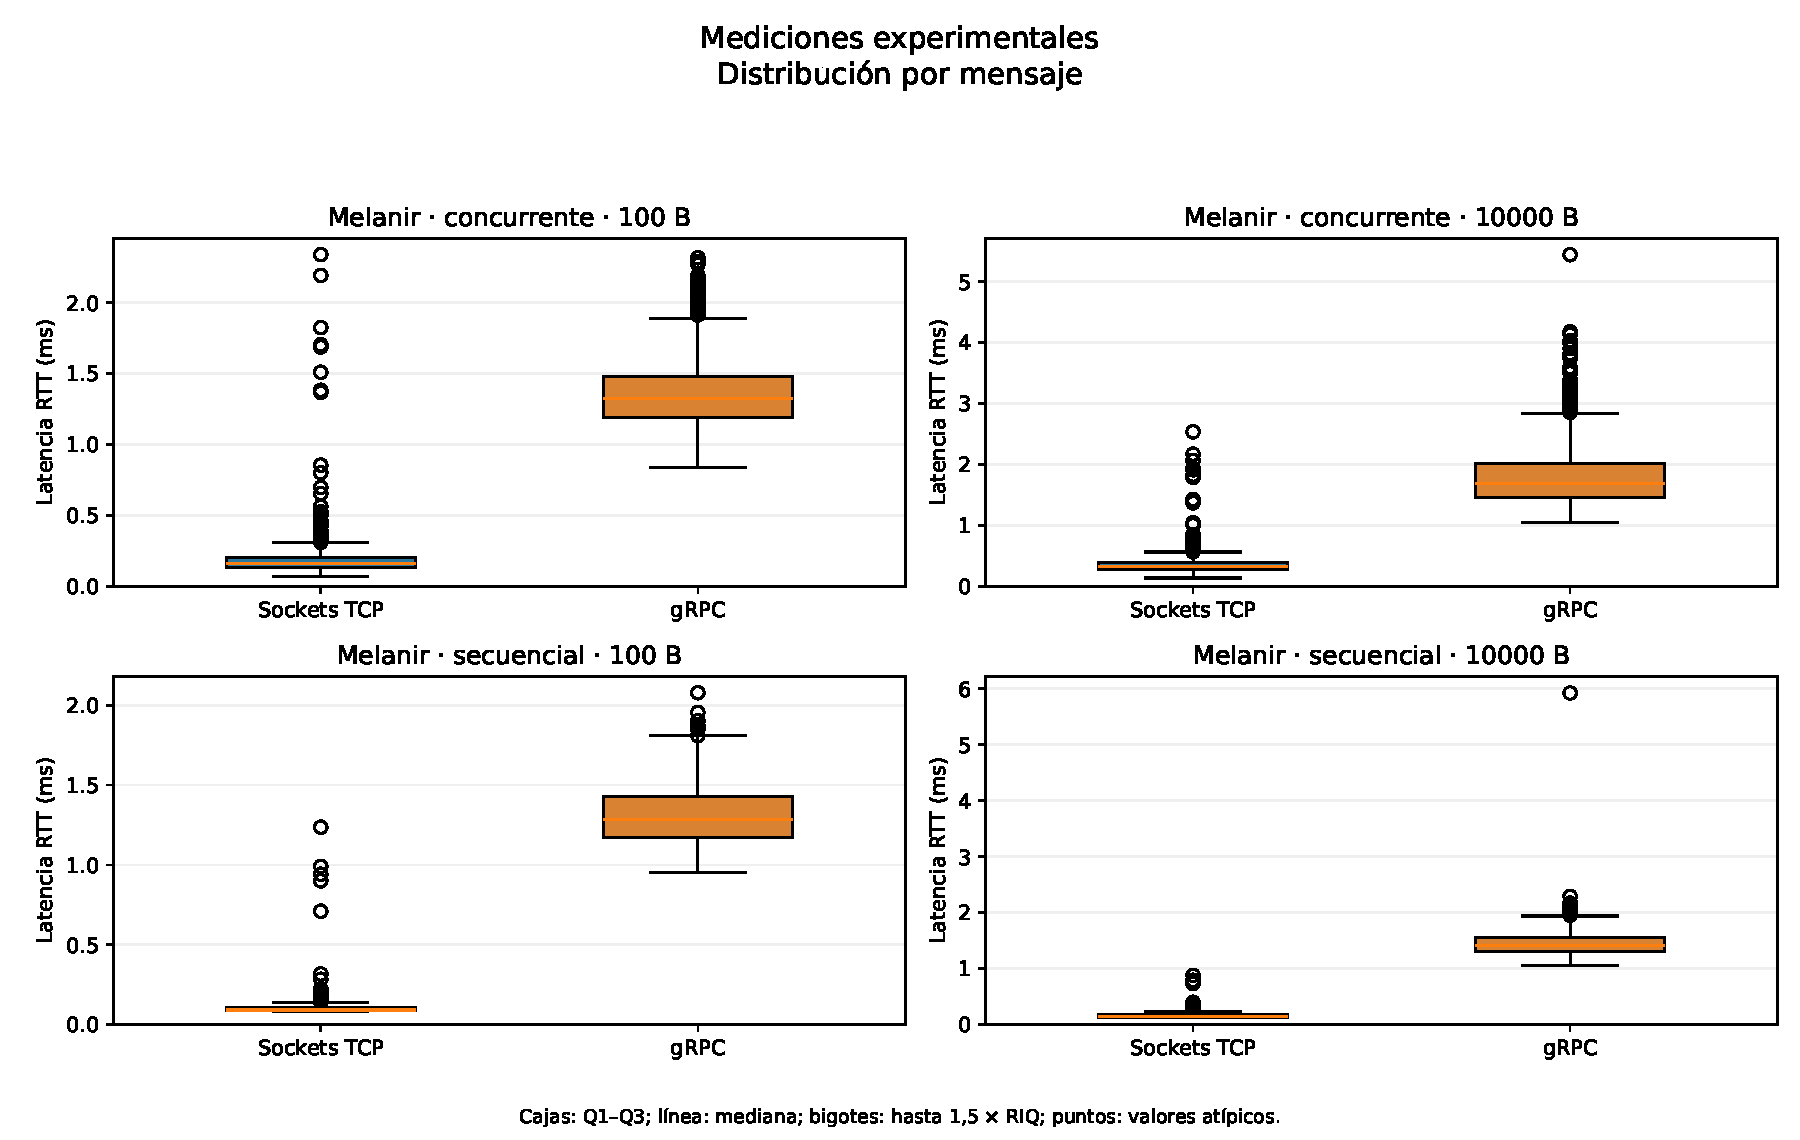
\includegraphics[width=\linewidth,height=0.80\textheight,keepaspectratio]{../analysis/resultados-finales-2026-11-22/melanie/cajas_latencias.pdf}
\caption{Distribución de las 8\,000 latencias válidas de Melanir,
separadas por mecanismo, modo y tamaño serializado.}
\label{fig:melanie-cajas}
\end{figure}
\begin{figure}[p]
\centering
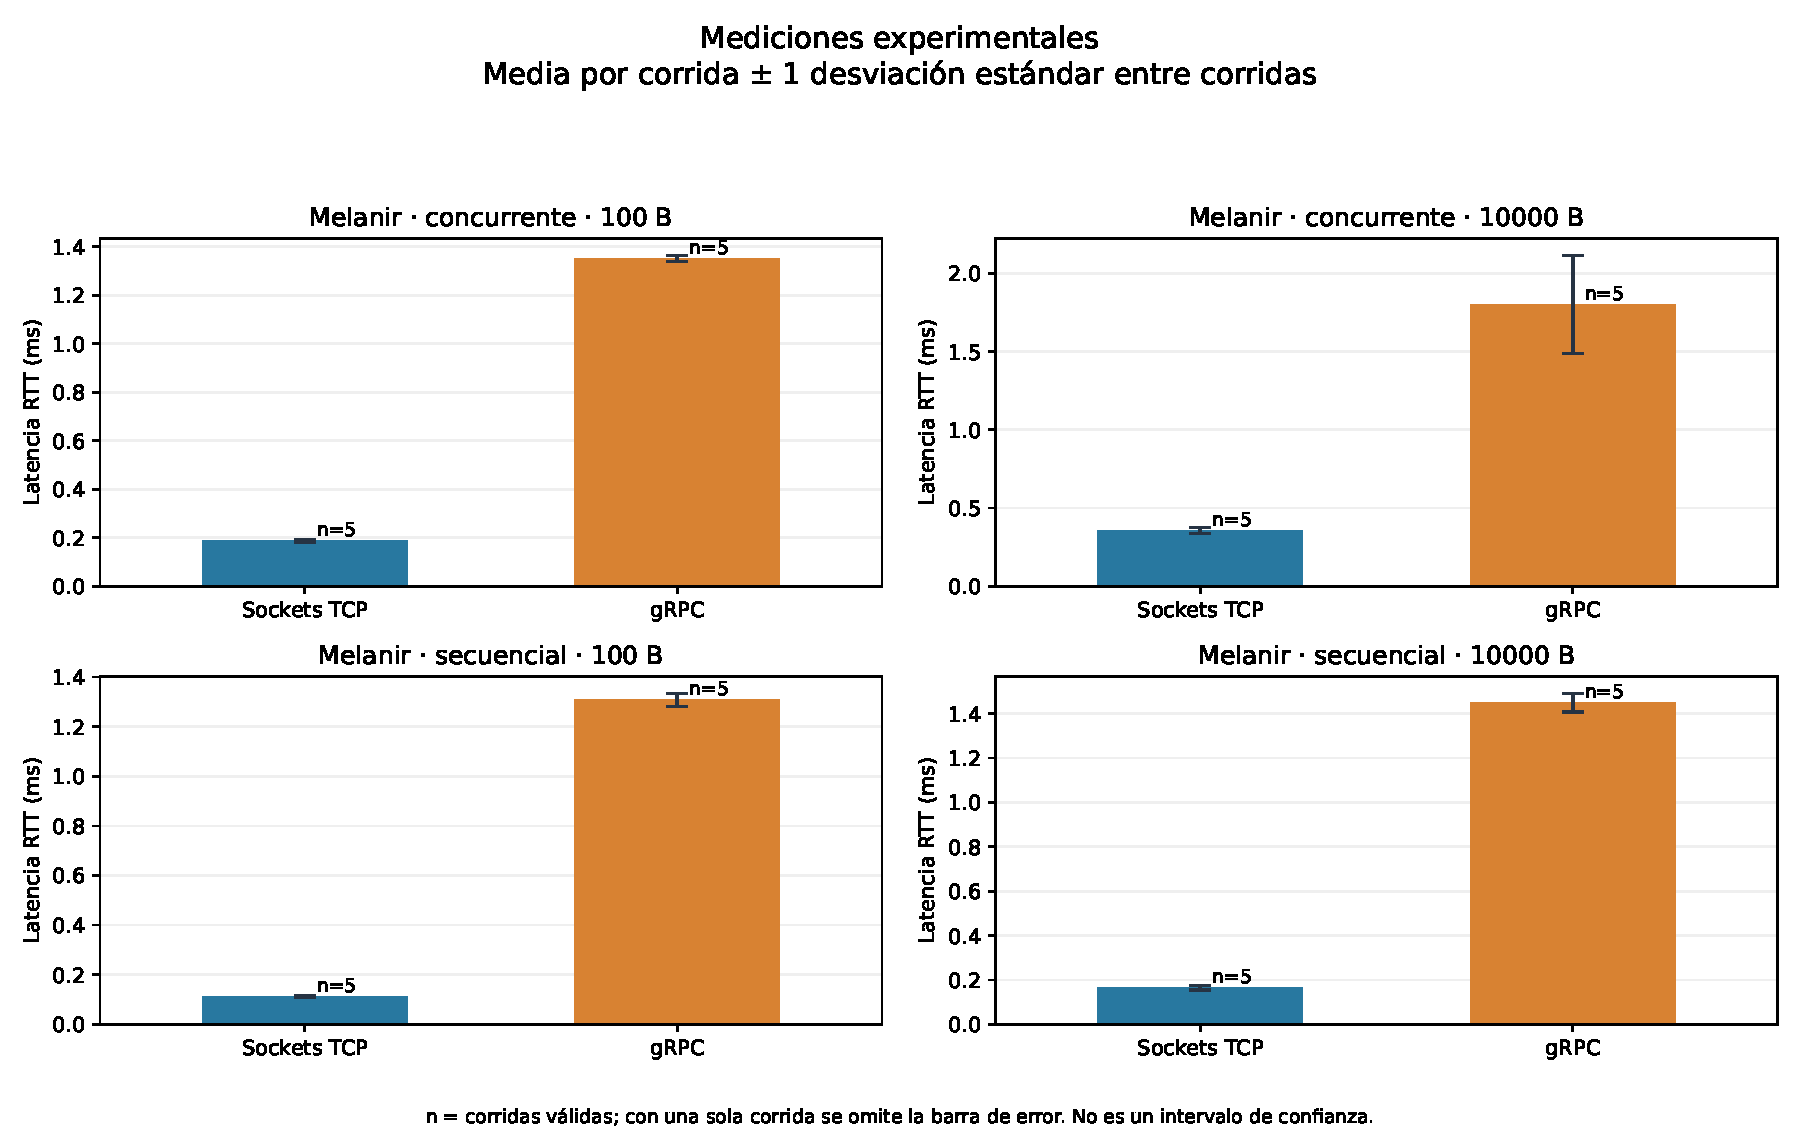
\includegraphics[width=\linewidth,height=0.80\textheight,keepaspectratio]{../analysis/resultados-finales-2026-11-22/melanie/barras_latencias.pdf}
\caption{Media de las medias de cinco corridas por condición en Melanir.
Las barras de error representan una desviación estándar muestral
entre corridas; no son intervalos de confianza.}
\label{fig:melanie-barras}
\end{figure}
\clearpage

\subsection{Orden lógico en los intercambios de esta sesión}
Las pruebas de intercambio de mensajes se ejecutaron aparte de las
corridas de latencia. Cada mecanismo produjo tres CSV, con 42 eventos
y 21 mensajes emparejados. El verificador comprobó 21 de 21 relaciones
envío--recepción y 42 de 42 actualizaciones locales en ambos casos.
Las evidencias corresponden a los eventos de aplicación de esta sesión
del 19/11, anterior a la corrección de los acuses. La verificación
posterior con acuses se presenta en el apartado~\ref{sec:lamport-ack}.

\begin{table}[htbp]
\centering\small
\caption{Ejemplos concurrentes encontrados en la sesión de Melanir.}
\begin{tabular}{llllr}
\toprule
Mecanismo & Nodo & Evento & Mensaje & Reloj \\
\midrule
Sockets & nodo-A & envío & \texttt{42dd864c} & 1 \\
Sockets & nodo-B & envío & \texttt{fe53befd} & 1 \\
gRPC & nodo-A & envío & \texttt{1c1cbfe3} & 1 \\
gRPC & nodo-B & envío & \texttt{93224eb9} & 1 \\
\bottomrule
\end{tabular}
\end{table}

En cada par, el recorrido de las relaciones locales y de los enlaces
de mensajes no encuentra un camino causal en ninguna dirección.
Los relojes iguales ilustran la concurrencia en estos registros;
las horas físicas no se usan para inferir el orden causal.

\subsection{Evidencia de ejecución en Melanir}
Las seis capturas siguientes se conservan sin modificaciones.
Las dos primeras sirven como apoyo de los procesos e intercambios
TCP: su encuadre no incluye toda la identificación.
Las cuatro restantes sí muestran usuario, equipo, fecha y hora.
La última documenta la ejecución del análisis conjunto.

\begin{landscape}
\begin{center}
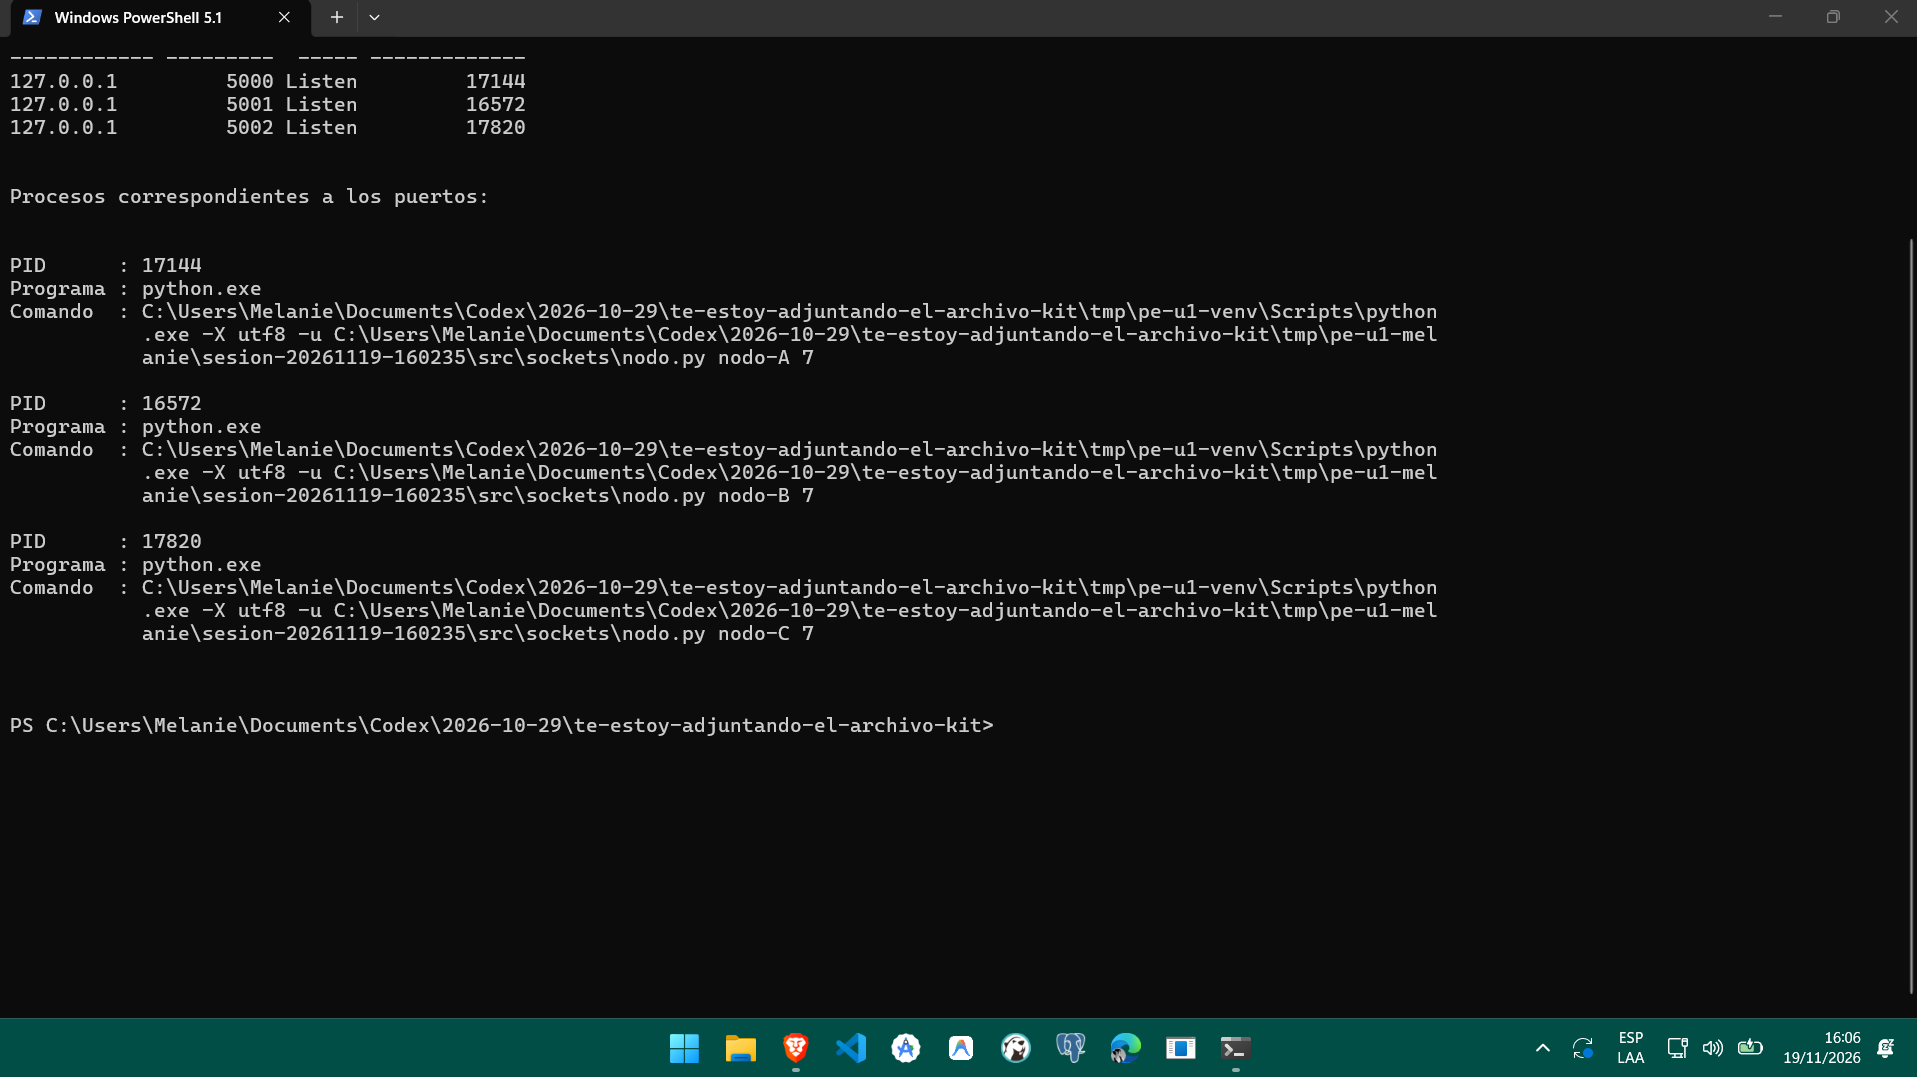
\includegraphics[width=\linewidth,height=0.85\textwidth,keepaspectratio]{../evidencias/melanie/2026-11-19/01-nodos-tcp.png}
\captionof{figure}{Procesos TCP escuchando en los puertos 5000, 5001 y 5002. Captura de apoyo.}
\end{center}
\end{landscape}
\begin{landscape}
\begin{center}
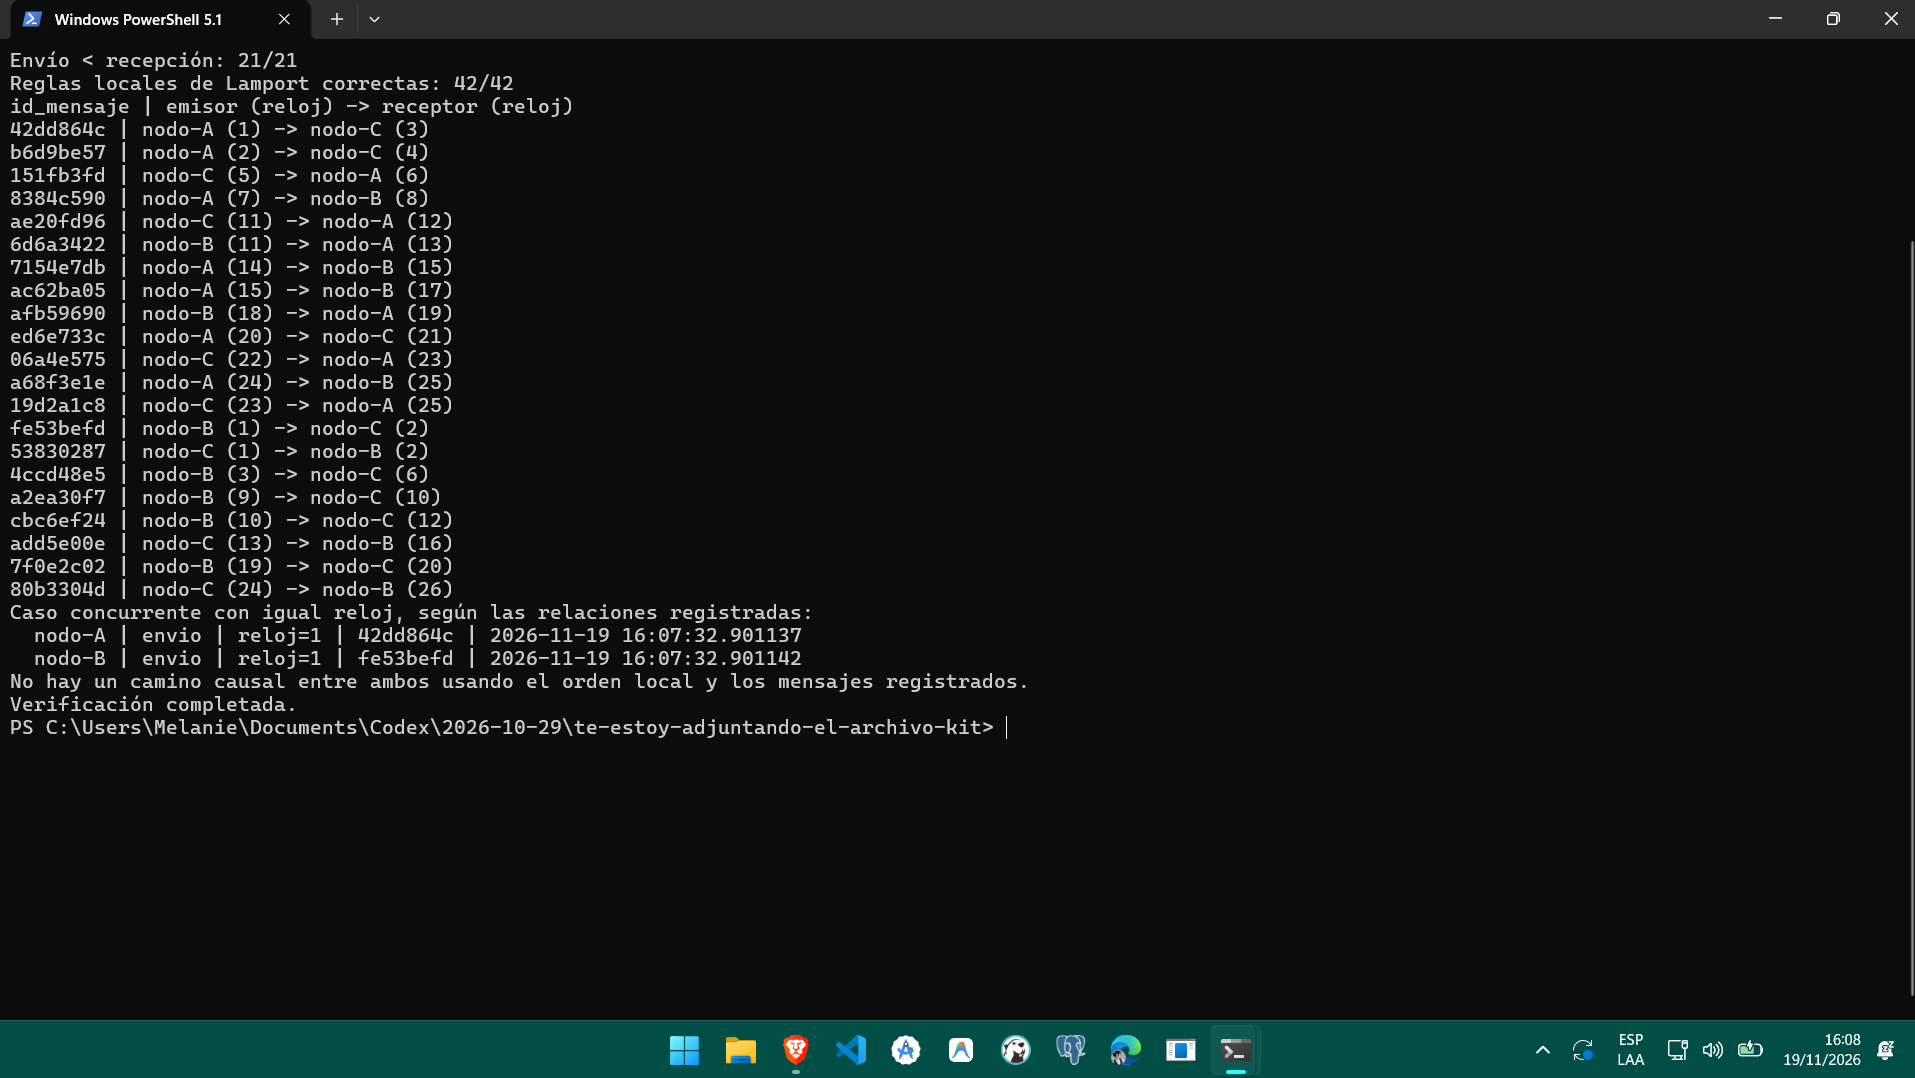
\includegraphics[width=\linewidth,height=0.85\textwidth,keepaspectratio]{../evidencias/melanie/2026-11-19/02-intercambios-tcp.png}
\captionof{figure}{Verificación de los intercambios TCP de la sesión. Captura de apoyo.}
\end{center}
\end{landscape}

\begin{landscape}
\begin{center}
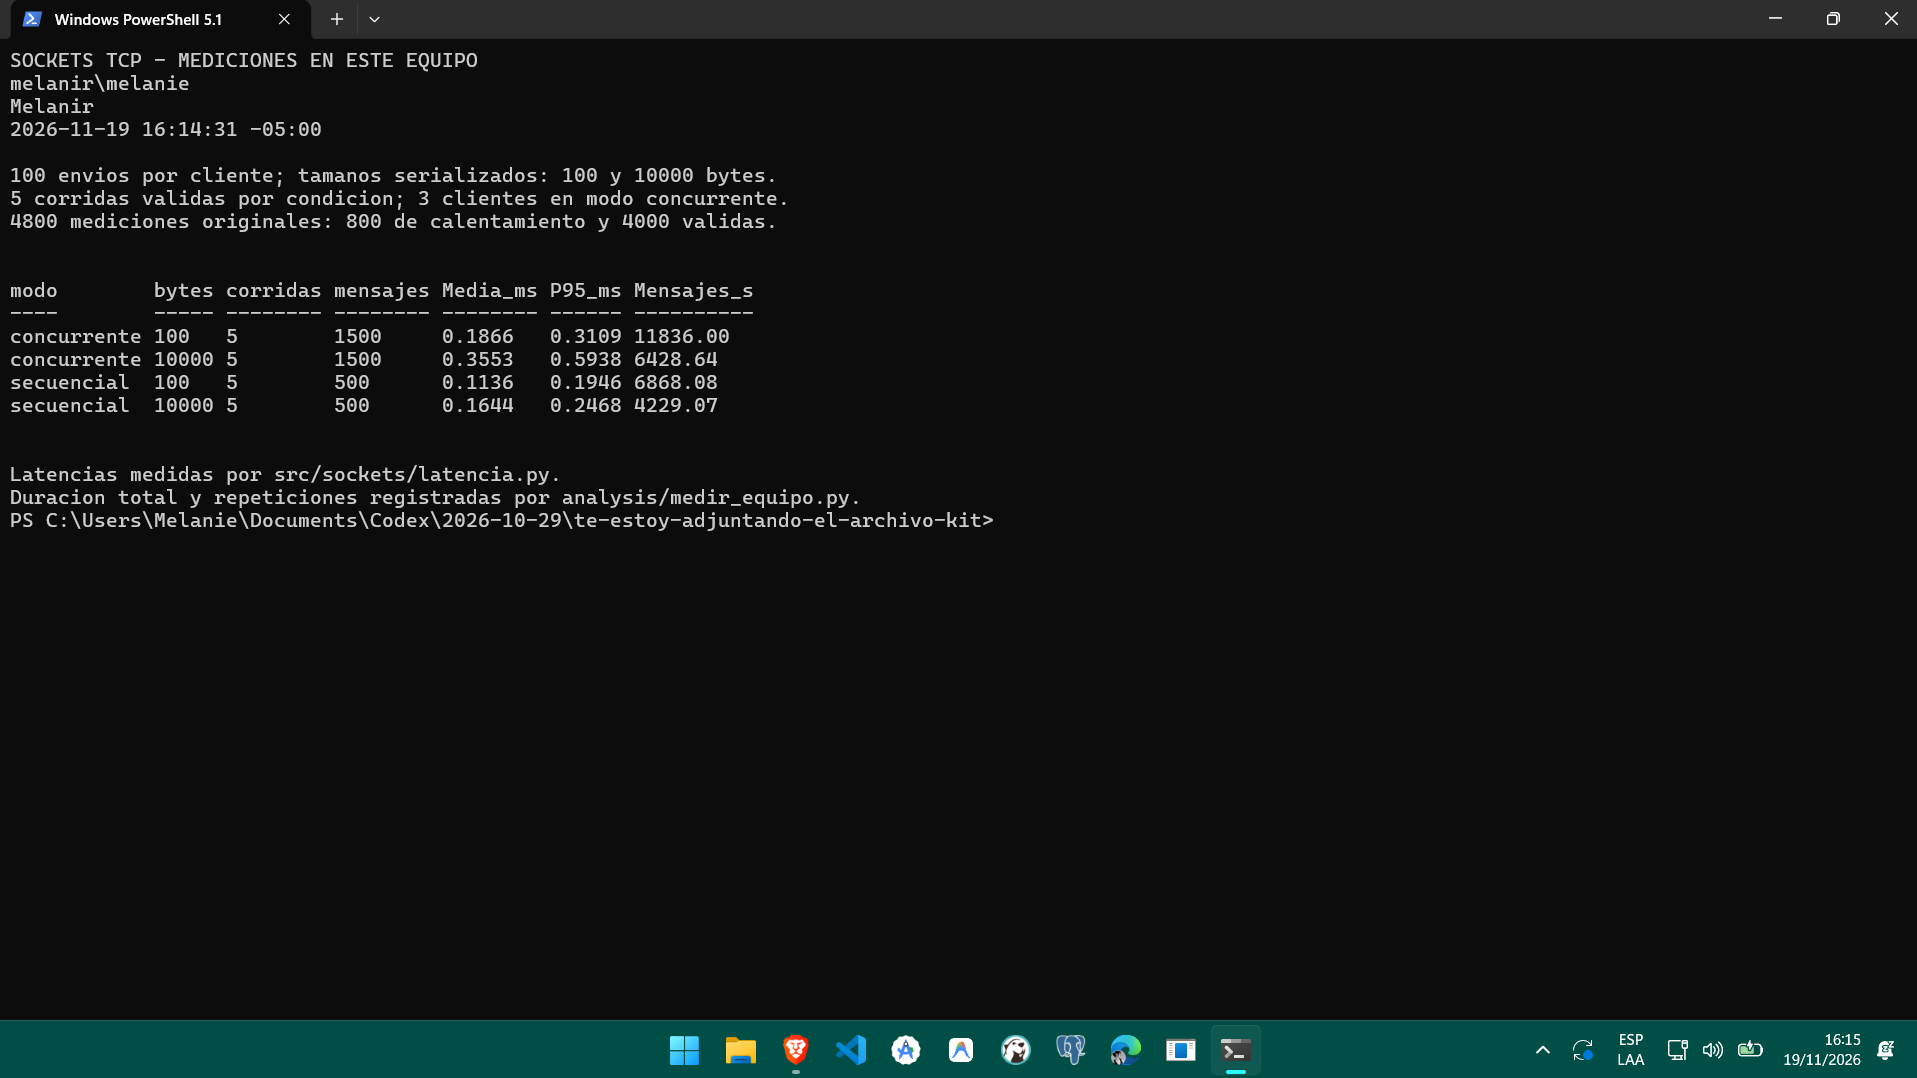
\includegraphics[width=\linewidth,height=0.85\textwidth,keepaspectratio]{../evidencias/melanie/2026-11-19/03-latencias-sockets.png}
\captionof{figure}{Resumen de las mediciones de sockets TCP en Melanir.}
\end{center}
\end{landscape}
\begin{landscape}
\begin{center}
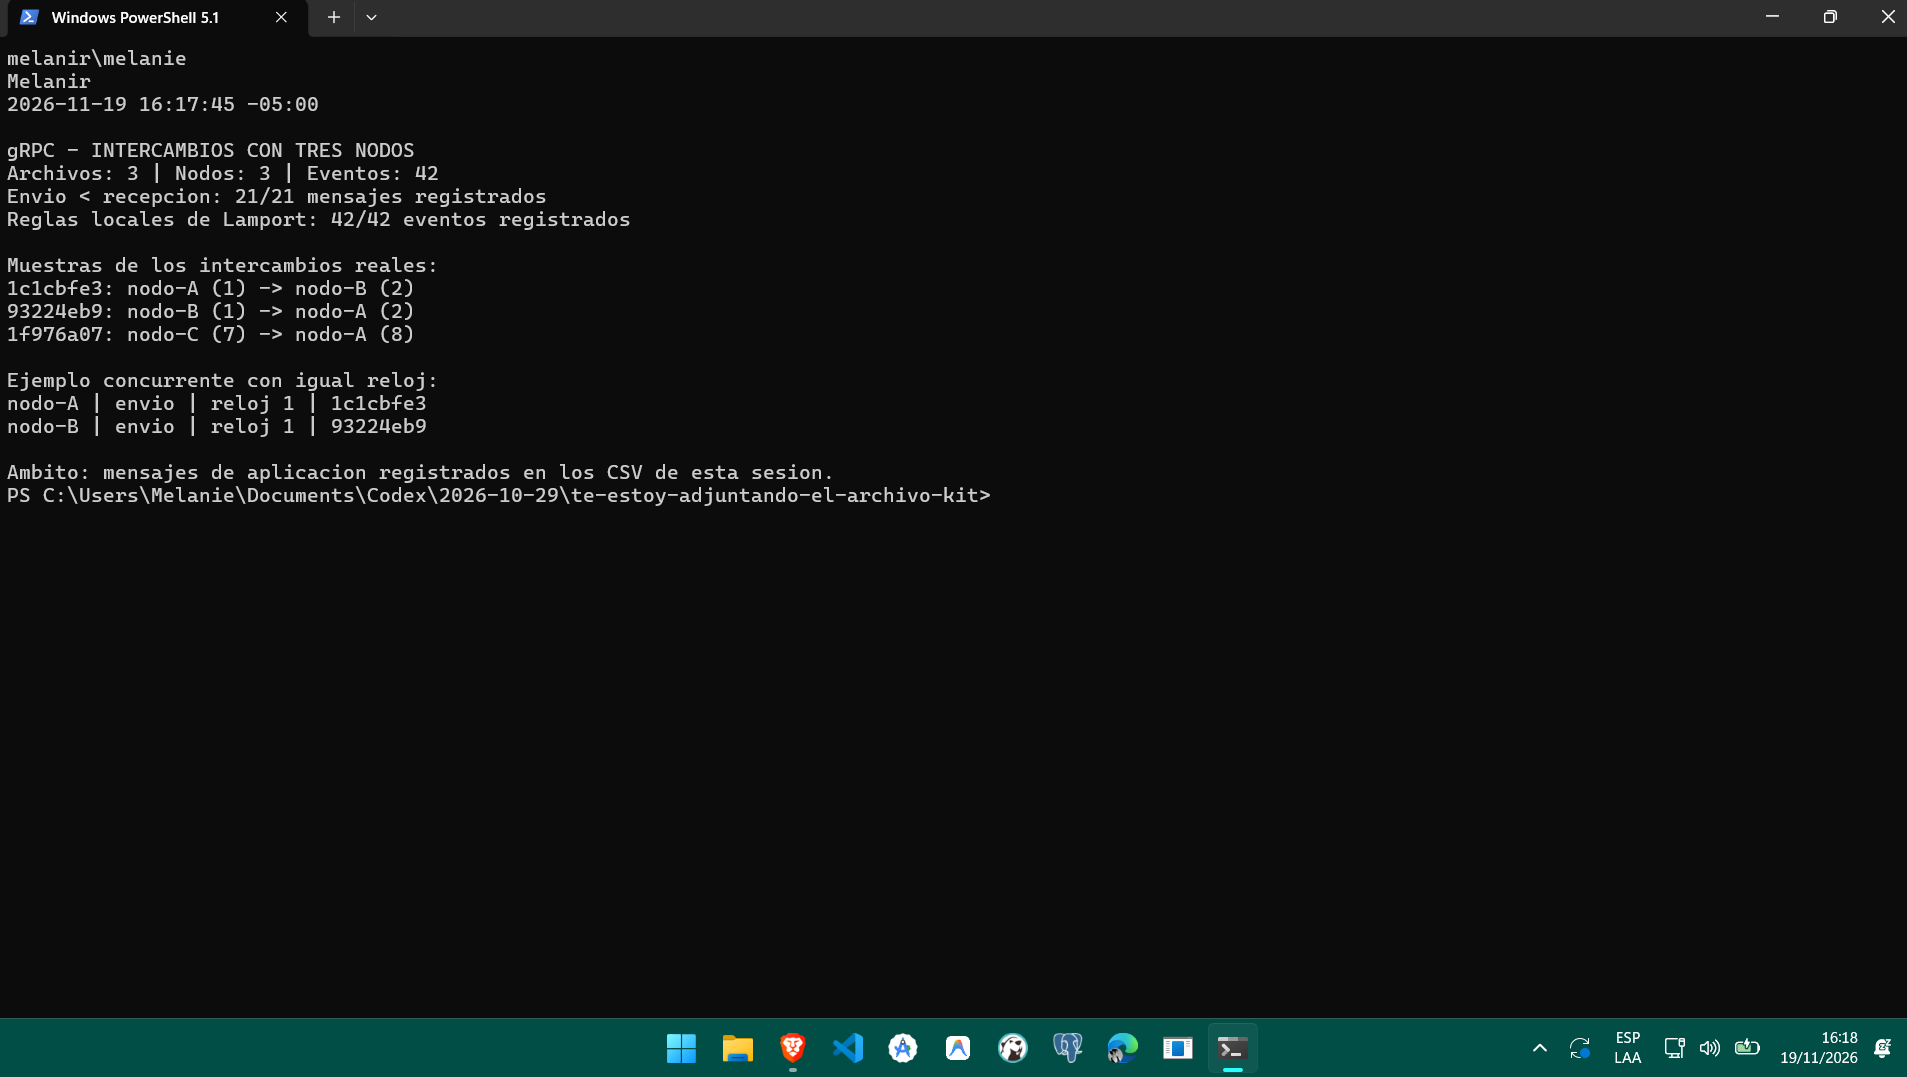
\includegraphics[width=\linewidth,height=0.85\textwidth,keepaspectratio]{../evidencias/melanie/2026-11-19/04-intercambios-grpc.png}
\captionof{figure}{Intercambios gRPC y verificación de los eventos de aplicación registrados.}
\end{center}
\end{landscape}
\begin{landscape}
\begin{center}
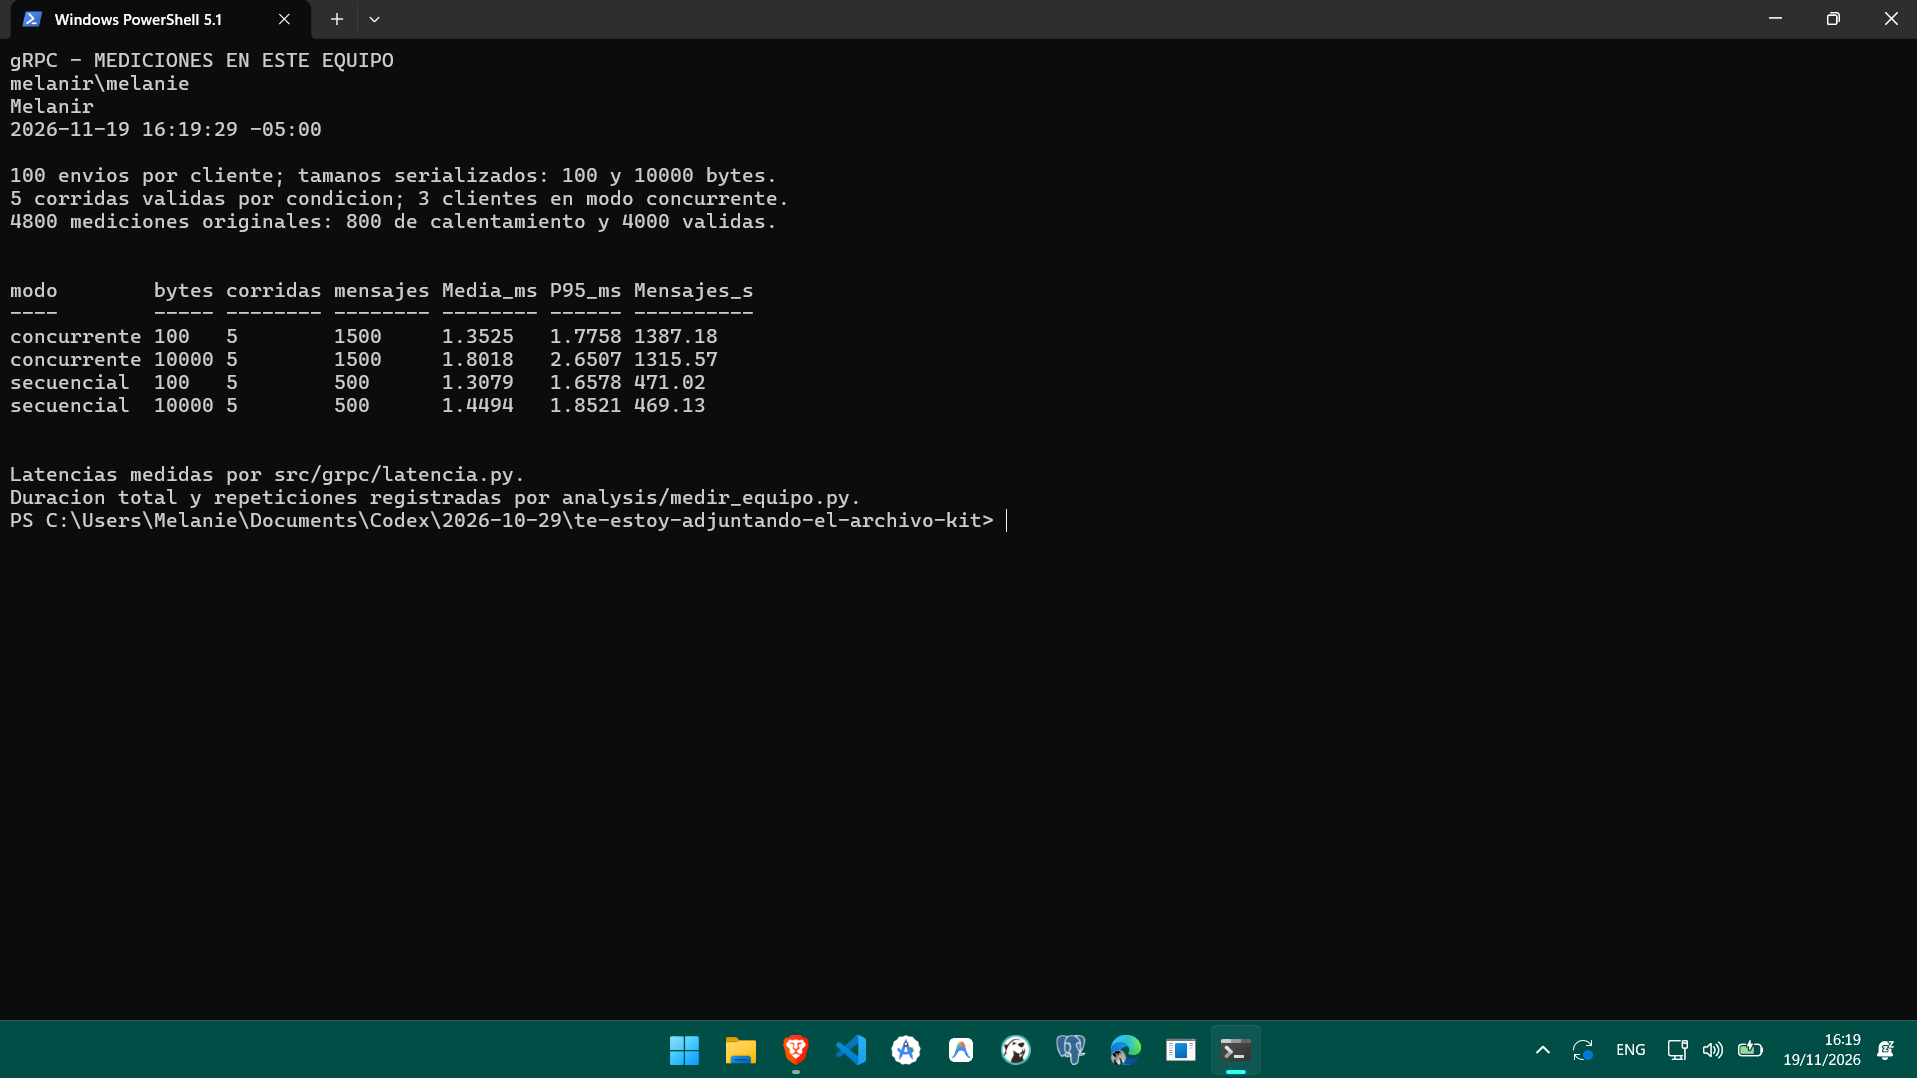
\includegraphics[width=\linewidth,height=0.85\textwidth,keepaspectratio]{../evidencias/melanie/2026-11-19/05-latencias-grpc.png}
\captionof{figure}{Resumen de las mediciones de gRPC en Melanir.}
\end{center}
\end{landscape}
\begin{landscape}
\begin{center}
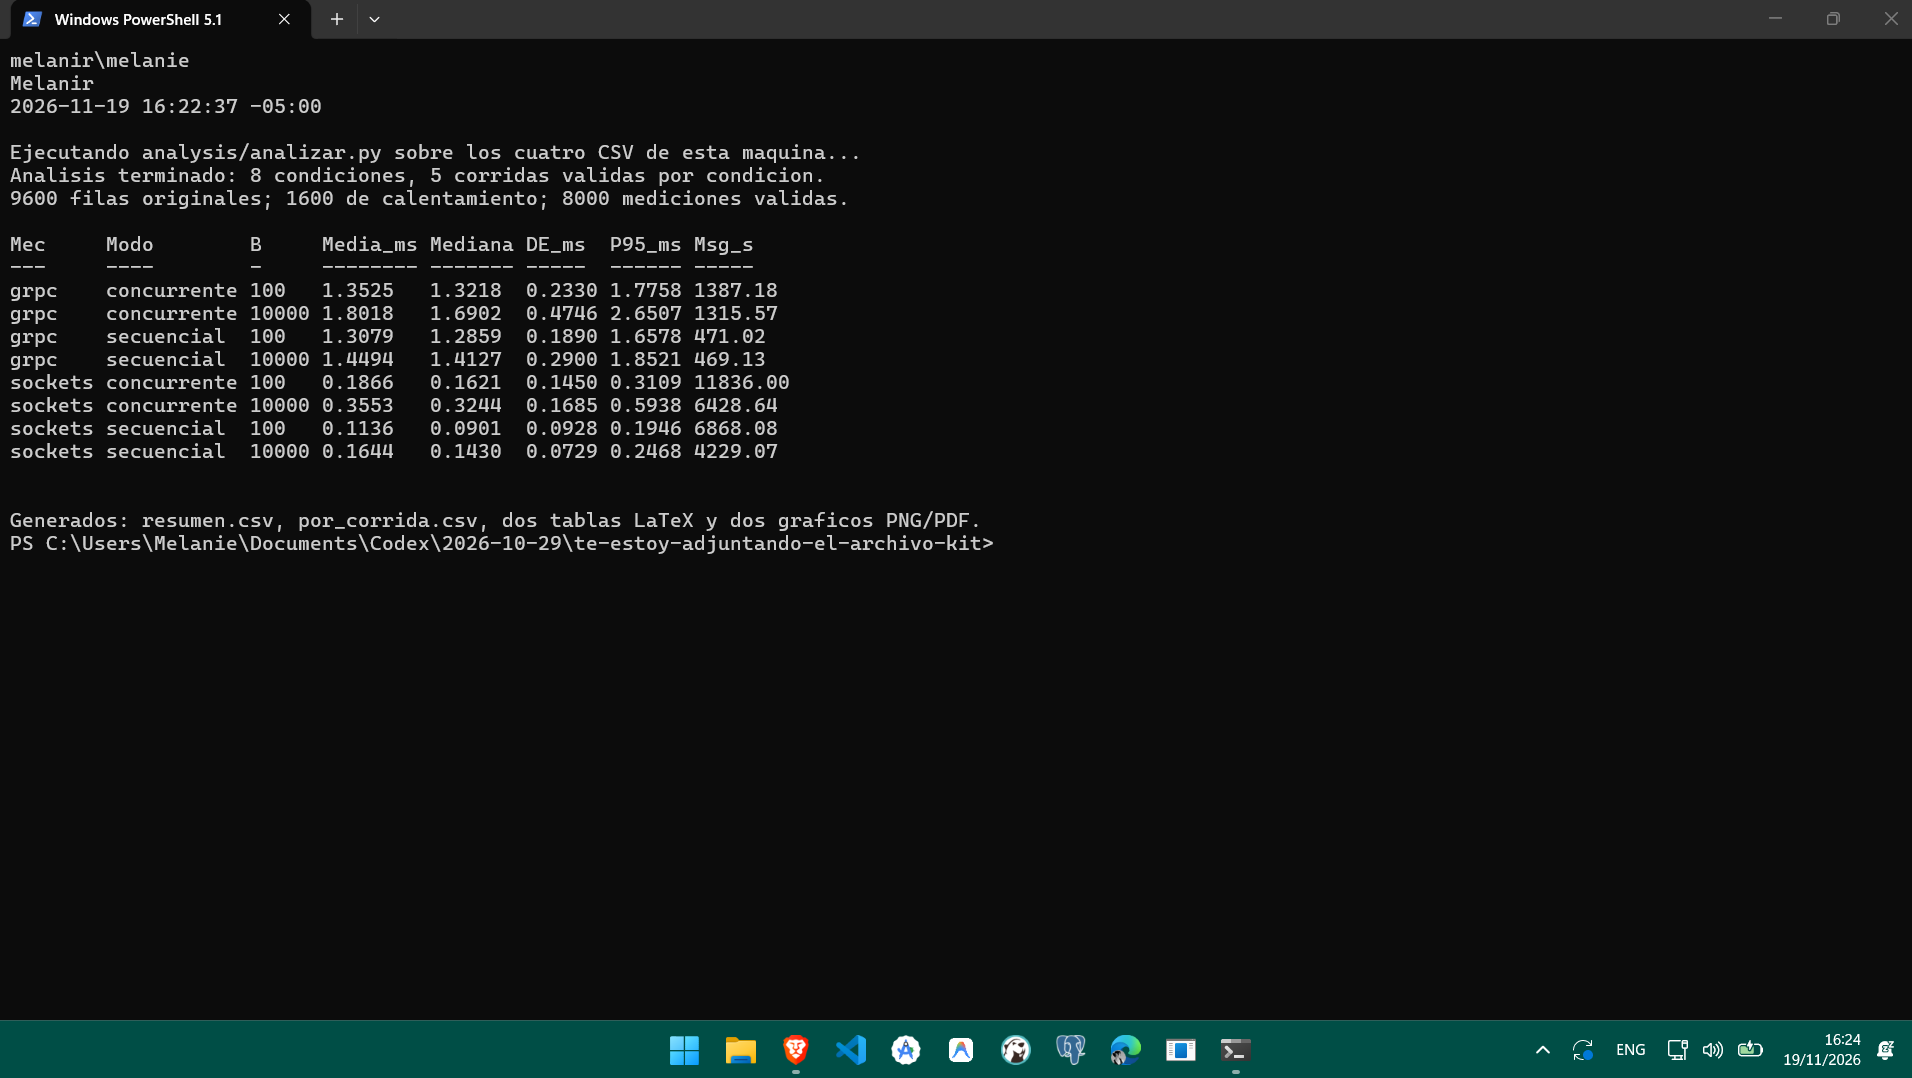
\includegraphics[width=\linewidth,height=0.85\textwidth,keepaspectratio]{../evidencias/melanie/2026-11-19/06-analisis-conjunto.png}
\captionof{figure}{Análisis conjunto de los cuatro CSV: ocho condiciones y 8\,000 mediciones válidas.}
\end{center}
\end{landscape}
